% ------------------------------------------------------------------------------
% TYPO3 CMS 8 LTS - What's New - Chapter "Introduction" (English Version)
%
% @author	Michael Schams <schams.net>
% @license	Creative Commons BY-NC-SA 3.0
% @link		http://typo3.org/download/release-notes/whats-new/
% @language	English
% ------------------------------------------------------------------------------
% LTXE-CHAPTER-UID:		7fdf26cc-362160ab-d6c8b905-19722b20
% LTXE-CHAPTER-NAME:	Introduction
% ------------------------------------------------------------------------------

\section{Introduction}
\begin{frame}[fragile]
	\frametitle{Introduction}

	\begin{center}\huge{\color{typo3darkgrey}\textbf{Introduction}}\end{center}
	\begin{center}\large{\textit{Quick overview of the facts}}\end{center}

\end{frame}

% ------------------------------------------------------------------------------
% LTXE-SLIDE-START
% LTXE-SLIDE-UID:		344cc625-72176049-0721f1aa-0580f11a
% LTXE-SLIDE-TITLE:		TYPO3 CMS 8 LTS - The Facts
% ------------------------------------------------------------------------------
\begin{frame}[fragile]
	\frametitle{Introduction}
	\framesubtitle{TYPO3 v8 LTS}

	\begin{itemize}
		\item Release date: 4 April 2017
		\item Release type: LTS Release (Long Term Release)
		\item Development time: 18+ months
	\end{itemize}

	\begin{figure}
		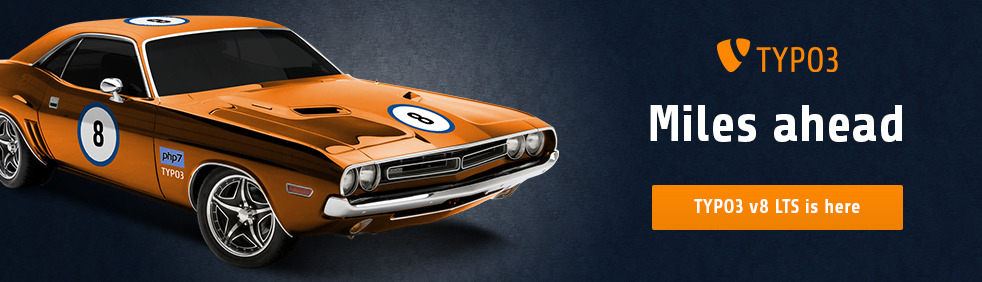
\includegraphics[width=0.95\linewidth]{Introduction/typo3cms87-banner.jpg}
	\end{figure}

\end{frame}

% ------------------------------------------------------------------------------
% LTXE-SLIDE-START
% LTXE-SLIDE-UID:		59b04868-09a761b3-0c7ca4c3-ce6e31bb
% LTXE-SLIDE-TITLE:		System Requirements (1)
% ------------------------------------------------------------------------------
\begin{frame}[fragile]
	\frametitle{Introduction}
	\framesubtitle{System Requirements (1)}

%	\vspace{-0.2cm}
%	\begin{figure}\raggedleft
%		
\includegraphics[width=0.15\linewidth]{Introduction/logo-php7.png}
%	\end{figure}

	\begin{columns}[T]

		\begin{column}{.75\textwidth}
			\tabto{0.1cm}
				\begin{itemize}
					\item PHP 7.0 is the minimum requirement\newline
						for TYPO3 v8 LTS
					\item Subsequent PHP 7 releases will be supported as they are released
					\item PHP 7 provides a significant performance boost
					\item Allows usage of new PHP 7 specific features

				\end{itemize}
		\end{column}

        \begin{column}{.25\textwidth}
			
\includegraphics[width=0.5\linewidth]{Introduction/logo-php7.png}
        \end{column}

    \end{columns}

	\begin{itemize}
		\item Required PHP settings:

			\begin{itemize}
				\item \texttt{memory\_limit} >= 128M
				\item \texttt{max\_execution\_time} >= 240s
				\item \texttt{max\_input\_vars} >= 1500
				\item compilation option \texttt{-}\texttt{-disable-ipv6} must \underline{not} be used
			\end{itemize}
	\end{itemize}


\end{frame}

% ------------------------------------------------------------------------------
% LTXE-SLIDE-START
% LTXE-SLIDE-UID:		ed65fc3f-293c3606-42f80134-5f1d7503
% LTXE-SLIDE-TITLE:		System Requirements (2)
% ------------------------------------------------------------------------------
\begin{frame}[fragile]
	\frametitle{Introduction}
	\framesubtitle{System Requirements (2)}

	\begin{itemize}
		\item TYPO3 v8 LTS uses \textbf{Doctrine DBAL}. All database servers
			supported by this DB abstraction layer are also supported by TYPO3.\newline
			For example:
	\end{itemize}

	\vspace{-0.4cm}
	\begin{figure}
		
\includegraphics[width=0.70\linewidth]{Introduction/logo-databases.png}
	\end{figure}

	\begin{itemize}

		\item Minimum disk space required: 200 MB
		\item The backend requires Microsoft Internet Explorer 11 or later,
			Microsoft Edge, Google Chrome, Firefox, Safari or any other modern,
			compatible browser

	\end{itemize}

\end{frame}


% ------------------------------------------------------------------------------
% LTXE-SLIDE-START
% LTXE-SLIDE-UID:		41f1b51a-6b837f9d-c4aa9584-66f8e47f
% LTXE-SLIDE-TITLE:		Sprint Releases
% ------------------------------------------------------------------------------
\begin{frame}[fragile]
	\frametitle{Introduction}
	\framesubtitle{Development Timeline}

	Sprint Releases published:

	\begin{itemize}
		\item v8.0 \tabto{1.1cm}22/Mar/2016\tabto{3.4cm}Fluid Standalone Engine
		\item v8.1 \tabto{1.1cm}03/May/2016\tabto{3.4cm}Cloud Integration
		\item v8.2 \tabto{1.1cm}05/Jul/2016\tabto{3.4cm}Doctrine Prerequisites
		\item v8.3 \tabto{1.1cm}30/Aug/2016\tabto{3.4cm}Rich Text Editor
		\item v8.4 \tabto{1.1cm}18/Oct/2016\tabto{3.4cm}Doctrine Migration + Upgrades
		\item v8.5 \tabto{1.1cm}20/Dec/2016\tabto{3.4cm}New RTE + Integrator Support
		\item v8.6 \tabto{1.1cm}14/Feb/2017\tabto{3.4cm}Cropping, Link Handling etc.
		\item v8.7 \tabto{1.1cm}04/Apr/2017\tabto{3.4cm}LTS Preparation and Release
	\end{itemize}

\end{frame}

% ------------------------------------------------------------------------------
% LTXE-SLIDE-START
% LTXE-SLIDE-UID:		f7c981ac-f359aac8-f8799a73-2adc6532
% LTXE-SLIDE-TITLE:		LTS Support Timeline
% ------------------------------------------------------------------------------
\begin{frame}[fragile]
	\frametitle{Introduction}
	\framesubtitle{Long Term Support}

	Maintenance/support timeline:

	\begin{figure}
		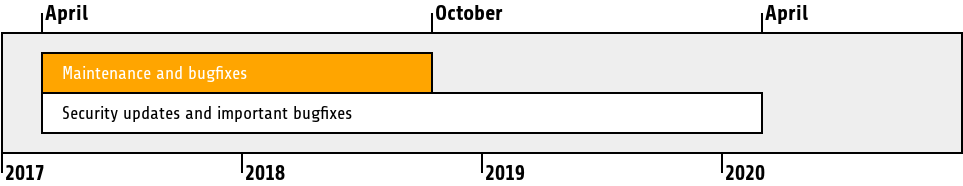
\includegraphics[width=1\linewidth]{Introduction/maintenance-support-timeline.png}
	\end{figure}

	\begin{itemize}
		\item TYPO3 version 8.7 is a LTS Release (Long Term Support)
		\item Regular maintenance and bugfixes until October 2018
		\item Security and critical bugfixes until April 2020
	\end{itemize}

\end{frame}

% ------------------------------------------------------------------------------
